\documentclass[tikz,border=5mm,12pt]{standalone}
\usepackage[fontsize=16pt]{fontsize}
\usetikzlibrary{arrows.meta}

\def\ysep{6mm}
\def\xsep{18mm}
\def\textYsep{22pt}
\def\labelXsep{24mm}
\def\vertEquiv{\rotatebox{90}{$\equiv$}}
\def\lgray{gray!50!lightgray}

\begin{document}
  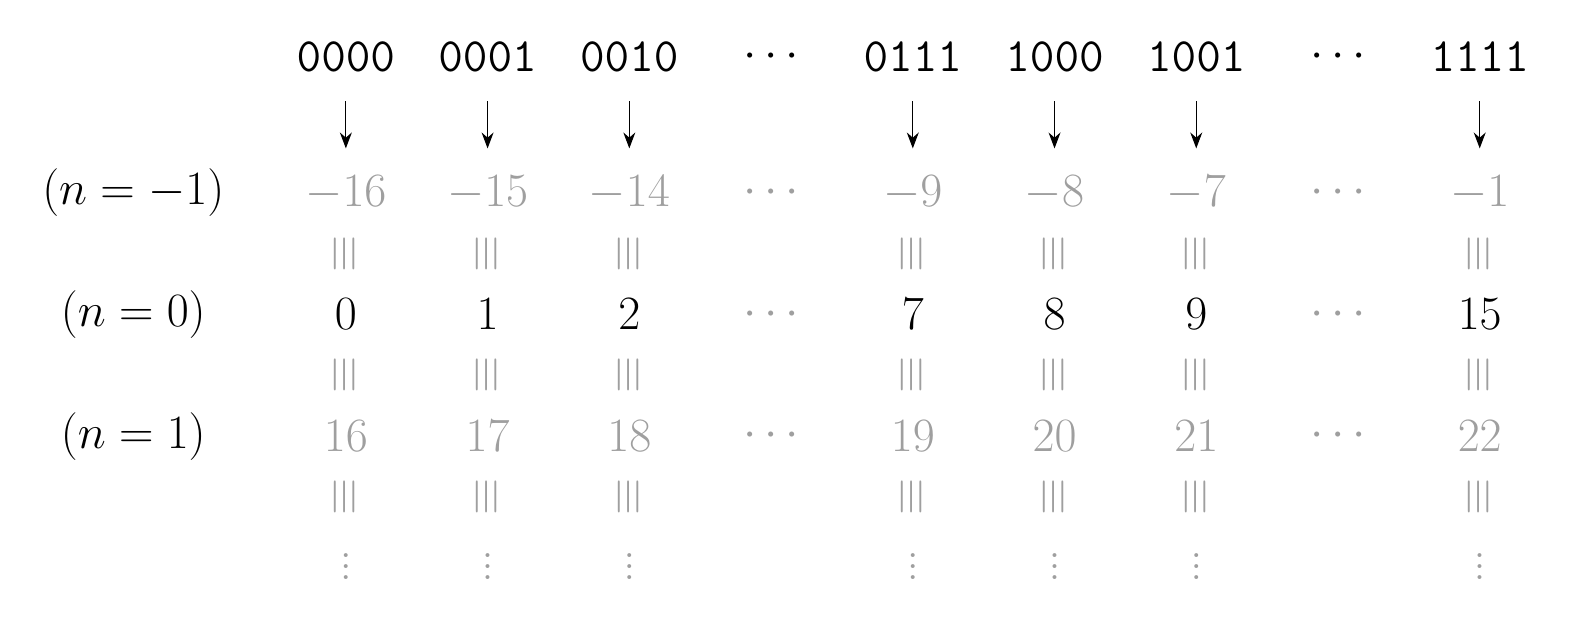
\begin{tikzpicture}[
    arrowtip/.style={
      -{Stealth[scale=1.2]}
    }
  ]
    \def\columns{
      0/0000/-16/\lgray/0/black/16/\lgray,
      1/0001/-15/\lgray/1/black/17/\lgray,
      2/0010/-14/\lgray/2/black/18/\lgray,
      4/0111/-9/\lgray/7/black/19/\lgray,
      5/1000/-8/\lgray/8/black/20/\lgray,
      6/1001/-7/\lgray/9/black/21/\lgray,
      8/1111/-1/\lgray/15/black/22/\lgray
    }

    \foreach \x / \label / \numA / \colorA / \numB / \colorB / \numC / \colorC in \columns {
      \node at (\x*\xsep,0pt) {\texttt{\label}};
      \draw[arrowtip] (\x*\xsep,-16pt) -- ++(0,-\ysep);
      \node[color=\colorA]   at (\x*\xsep,-\ysep-10pt-1*\textYsep) { $\numA$ };
      \node[color=\lgray] at (\x*\xsep,-\ysep-10pt-2*\textYsep) { \vertEquiv };
      \node[color=\colorB]   at (\x*\xsep,-\ysep-10pt-3*\textYsep) { $\numB$ };
      \node[color=\lgray] at (\x*\xsep,-\ysep-10pt-4*\textYsep) { \vertEquiv };
      \node[color=\colorC]   at (\x*\xsep,-\ysep-10pt-5*\textYsep) { $\numC$ };
      \node[color=\lgray] at (\x*\xsep,-\ysep-10pt-6*\textYsep) { \vertEquiv };
      \node[color=\lgray] at (\x*\xsep,-\ysep-10pt-7*\textYsep) { $\vdots$ };
    }

    \def\dotsColumns{3,7}

    \foreach \x in \dotsColumns {
      \node at (\x*\xsep,0) { $\cdots$ };
      \node[color=\lgray] at (\x*\xsep,-\ysep-10pt-1*\textYsep) { $\cdots$ };
      \node[color=\lgray] at (\x*\xsep,-\ysep-10pt-3*\textYsep) { $\cdots$ };
      \node[color=\lgray] at (\x*\xsep,-\ysep-10pt-5*\textYsep) { $\cdots$ };
    }

    \def\leftLabels{-1,0,1}

    \foreach \label [count=\i] in \leftLabels {
      \node at (-1.5*\xsep,-\ysep-10pt+\textYsep-2*\i*\textYsep) { ($n=\label$) };
    }
  \end{tikzpicture}
\end{document}
